\chapter{Fonctionnalités}

\section{Les tâches principales}

\subsection{Se déplacer}

Le déplacement est bien entendu un élément cruciale de la conception
d'un robot. La desserte robotisée a ceci de particulier qu'elle doit
évoluer en milieu humain. Cela demande de définir exactement quand le
robot est en risque de rencontrer des humains, et comment il doit
réagir.

Au dela de cet aspect, nous devons également définir tous les types de
déplacements que le robot devra effectuer:

\begin{itemize}
\item Construction de carte
\item arrivée en salle
\item déambulation
\item gestion de groupe
\item suivi
\item dirigé
\item retour à la base
\item utilisation de l'interface
\end{itemize}

\subsubsection{Mode construction de carte}
La construction de carte est l'action primaire du robot lui permettant par la suite de se repérer dans la salle. C'est pourquoi elle doit se dérouler avant l'arrivée des convives ou après leur départ. C'est durant cette phase que le robot crée un carte de la salle de cocktail dans laquelle il va devoir se déplacer. Ainsi, lors de la réception, il pourra savoir se positionner dans la salle de réception.

La phase de construction de carte se déclenche par un élément externe comme le maître de réception. Pour déclencher se mode il faut que le robot soit dans la salle à cartographier. C'est à dire que le robot peut y être présent avant le lancement d'un autre mode de déplacement ou après avoir suivi la personne qui enclenchera le mode, soit après le mode suivi.

la cartographie se réalise à l'aide de deux caméra. Le robot se déplace seulement pour peaufiner sa carte. Sinon le robot tourne sur lui-même pour réaliser sa carte de repère. Ce mode se termine lorsque le robot a réalisé sa carte. 

Après avoir enclenché réalisé la carte, le robot devra rentrer à sa base avant le lancement de la soirée cocktail.

Les points d'entrées du mode sont:
\begin{itemize}
\item aucun mode
\item Le mode suivi
\end{itemize}

Les points de sorties du mode sont:
\begin{itemize}
\item le mode retour à la base.
\end{itemize}

\subsubsection{Mode arrivée en salle}

Le déplacement de la base vers la salle est la première chose que doit réaliser 
le robot avant de commencer sa déambulation. C’est donc  le moment où il vérifie 
que ses batteries sont chargées, que son plateau est rempli et qu’il connait le 
chemin vers la salle. Le mouvement de la base vers la salle peut être déjà cartographié.
Cet évènement ne peut arriver que s’il est déjà à sa base.

Les points d'entrées du mode sont:
\begin{itemize}
\item Le mode retour à la base
\item Le mode dirigé
\item Le mode suivi
\end{itemize}

Les points de sorties du mode sont:
\begin{itemize}
\item le mode déhambulation.
\end{itemize}


\subsubsection{Mode déambulation}

Le mode déambulation est l'un des princpaux mode de déplacement de la
desserte. Il s'agit pour le robot de repérer un groupe de convive puis
de se déplacer vers lui. Un des point clé de ce déplacement est que le
robot doit éviter de retourner sur une zone géographique qu'il à déjà
servi.

le déroulement du mode se fait comme suit:
\begin{itemize}
\item déclenchement du mode à l'arrivée dans la salle.
\item la disserte va de groupe en groupe et le cas échéant de table en
  table.
\item le robot garde en mémoire les zones géographiques déjà
  desservies et priorise les zones encore non servie.
\item Fin du mode de déambulation à la fin d'un timer et/ou après une
  diminution significative du poids du plateau, ou en cas d'absence
  d'espace ou passer (interieur d'un groupe), ou en cas de rencontre
  d'un groupe.\\
\end{itemize}

les points d'entrée du mode sont:
\begin{itemize}
\item le mode utilsation de l'interface
\item le mode arrivée en salle
\item le mode suivi
\item le mode dirigé\\
\end{itemize}

les points de sorties du mode sont:
\begin{itemize}
\item le mode suivi
\item le mode dirigé
\item le mode retour à la base
\item le mode gestion de groupe
\item le mode utilisation de l'interface\\
\end{itemize}

\subsubsection{Mode gestion de groupe}
Le mode de gestion de groupe est destiné au service d'un groupe de personnes. Suite à la prise de décision du robot de servir un groupe qu'il a détecté. Celui-ci rentre dans ce mode avant d'effectuer le service. Celui-ci commence par déterminer une hiérarchie dans le groupe lui permettant d'établir l'ordre le plus efficace et socialement correct pour servir les convives. La sortie du mode s'effectue une fois le service terminée.\\

Les points d'entrées du mode sont :
\begin{itemize}
\item mode déambulation
\end{itemize}

Les points de sortie du mode sont :
\begin{itemize}
\item mode déambulation
\end{itemize}

\subsubsection{Mode suivi}
Le mode suivi est un mode qui peut uniquement être activé et désactivé de façon manuelle via le mode utilisation interface.
Celui-ci est destiné à une utilisation exceptionnelle pour des cas spéciaux.

On pourra imaginer un mécanisme de sécurité implémenté dans l'interface qui permettra uniquement à des personnes habilitée d'activer ce mode de déplacement.
Une fois le mode activer, un émetteur amovible sera libéré et mis à la disposition de la personne ayant activer le mode.
Après activation du mode, le robot suivra cette émetteur en gardant une certain distance de sécurité, afin qu'en évitant tout se qui pourrait venir se placer dans son chemin. Cela permet donc d'emmenner le robot à n'importe quel endroit souhaité, par exemple une zone de chargement spéciale éloigné de la base du robot.\\


Les points d'entrées du mode sont :
\begin{itemize}
\item mode utilisation interface
\end{itemize}

Les points de sortie du mode sont :
\begin{itemize}
\item mode utilisation interface
\end{itemize}

\subsubsection{Mode dirigé}
Le mode dirigé permet au robot de faire des dessertes spéciales transmise par l'ordinateur centrale.
Cet ordre peut avoir été passé par le maitre d'hotel tout comme par un convive, demandant à un certain robot de changer de section, ou bien d'aller deservir une table ou un groupe particulier.
On peut aussi envisager de lui faire livrer une commande spéciale.\\

Le déroulement du mode se fait comme suit:
\begin{enumerate}
\item Commande reçue par l'ordinateur centrale
\item L'ordinateur centrale determine le meilleur robot pour effectuer la desserte
\item Si besoin, le robot choisie va à sa base pour récupérer ce dont il à besoin
\item Le robot effectue la desserte demandé\\
\end{enumerate}


Les points d'entrées du mode sont :
\begin{itemize}
\item mode déambulation
\item mode arrivée en salle
\item mode retour à la base
\end{itemize}

Les points de sortie du mode sont :
\begin{itemize}
\item mode déambulation
\item mode arrivée en salle
\item mode retour à la base
\end{itemize}

\subsubsection{Mode retour a la base}

Ce mode permet au robot de rentrer à la base lorsqu'il en a besoin
(ravitaillement, disfonctionnement, rappel du maitre d'hotel...).

le déroulement du mode se fait comme suit:
\begin{itemize}
\item déclenchement lorsque le plateau est vide et/ou timer, en cas de
  detection d'anomalie, ou de rappel à la base.
\item en cas de déplacement impossible, envoie une demande demande
  d'assistance.
\item cherche le plus court chemin ne passant pas par des groupes
\item fin du mode lorsque le robot arrive à la base.\\
\end{itemize}

les points d'entrée du mode sont:
\begin{itemize}
\item le mode déambulation
\item le mode utilsation de l'interface
\item le mode arrivée en salle
\item le mode suivi
\item le mode dirigé\\
\end{itemize}

les points de sorties du mode sont:
\begin{itemize}
\item le mode suivi
\item le mode dirigé
\item le mode utilisation de l'interface\\
\end{itemize}

\subsubsection{Mode utilisation interface}
Le robot entre dans ce mode lorsque quelqu'un utilise une des
interfaces du robot. Dans ce cas le robot doit cesser de se deplacer.

\subsection{schéma générale}

\begin{figure}[h]
\begin{center}
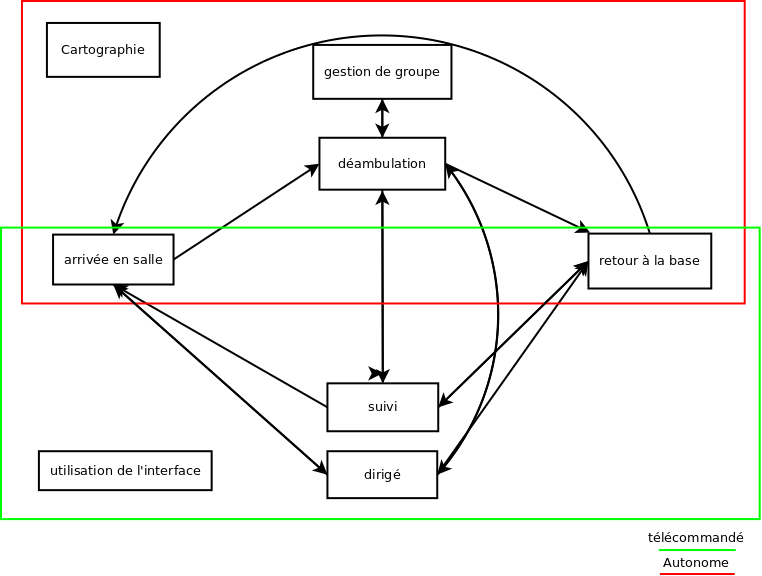
\includegraphics[scale=0.55]{Images/transition_mode.png}
\caption{Transition des modes}
\label{Transition des modes}
\end{center}
\end{figure}

\subsection{Servir}

Comme le mouvement, le service est un acte essentiel que doit pouvoir réaliser la desserte robotisée.
 La différence entre le service qu’un humain pourrait réaliser et celui que réalise le robot ne doit
 pas être remarqué par les invités du cocktail. Il est donc indispensable que ce service doit être le
 plus naturel possible. C’est dans la fluidité de l’action et la maintenue du plateau que le robot 
pourra créer une confiance envers les invités.

\subsubsection{Maintenir le plateau}

Pour maintenir le plateau efficacement, il doit rester le plus droit possible. Que ça soit lors du service ou lors de la déambulation, le plateau reste toujours le plus stable possible. 

Lors des déplacements, le plateau doit être en sécurité pour éviter d’être renversé. Il doit donc avoir une position de sécurité ou pouvoir être rangé par le robot de telle sorte qu’il ne subisse pas de chocs.

Lors d’un service dans un groupe, le plateau doit être le plus stable possible. Ainsi, les invités peuvent prendre avec confiance leurs aliments ou leurs verres sur le plateau.

%Peut être faire un petit point sur les deux modes

\subsubsection{Presenter le plateau}

La présentation d’un plateau se fait au niveau des coudes de l’invité qui se sert. C’est-à-dire que le plateau peut se trouver très haut, pour les grandes personnes, ou très bas, pour les enfants ou les personnes en fauteuil roulant. Pour prendre une moyenne, il faudrait que le plateau puisse se trouver entre 65cm au-dessus du sol et 1m30.

Le plateau n’a pas besoin de s’avancer dans un groupe lorsqu’il se présente. Il doit simplement se trouver à une hauteur idéale pour que la personne qui se fait servir puisse prendre ce qu’il y a sur le plateau sans être dérangé. S’il fait un geste en avant pour s’introduire dans un groupe, il risque de déranger des personnes en discussion parfois confidentiel. Le plateau a donc seulement un mouvement vertical pour le service.

La présentation à une durée limitée. Si les personnes ne se servent pas, le robot doit comprendre qu’ils ne sont pas à la recherche d’apéritifs et donc qu’il doit aller à la recherche d’un autre groupe. Si par contre les invités se servent, il faut que le robot attende que tout le monde soit servi et qu’il ait le droit de se retirer. Pour cela, il sait détecter quand personne ne prend d’éléments sur son plateau et a un timer qui vérifie qu’il ne reste pas inutilement à un endroit et qui lui dit de rester un certain moment avant de se retirer.

% peut être faire un subsection levé et descente du plateau de façon vertical et savoir quand se retirer ?

\subsection{Communication}
 
Pour permettre une bonne gestion de l’interaction entre l’homme et la machine, le robot doit pouvoir communiquer avec les invités. C’est dans son interface qu’il se démarquera des autres robots sur le marché.

Cette communication doit être basée sur la possibilité de se renseigner sur le cocktail en général. Il doit donc pouvoir donner les informations sur ce qui est et va être servi au cours du cocktail. De plus il doit savoir exactement de quoi son composé les différents mets.

Pour parfaire son utilité, il doit pouvoir indiquer à un invité un moyen de connaitre un autre invité. La réussite de cette fonctionnalité peut se faire par le fait d’amener l’invité vers celui qu’il cherche ou lui donné un indice pour le trouver comme une photo ou un nom.

Il peut aussi se rendre lui-même image de communication subtile en ayant la possibilité de changer de coque pour s’adapter au cocktail. Bien que le robot doive toujours rester noir pour rester dans l’ambiance d’un cocktail, il peut s’ajouter un logo ou un symbole pour le mettre en harmonie avec l’évènement.

%Pareil que pour les deux sous partie ultérieurs.
